% Устанавливаем размер шрифта в 14 пунктов.
% Рекомендованный размер шрифта по ГОСТ 7.32-2017 ---
% не менее 12 пунктов [1, §́ 6.1.1].
\documentclass[14pt,russian]{extarticle}

\usepackage{amsmath}

\usepackage[shortcuts]{extdash}
\usepackage{array}
\usepackage{graphicx}

\usepackage[math]{cellspace}
\cellspacetoplimit 4pt
\cellspacebottomlimit 4pt

% Настройка формат страниц и величины полей согласно [1, § 6.1.1].
\usepackage[
	a4paper,
	bindingoffset=0pt,
	left=30mm,
	right=15mm,
	top=20mm,
	bottom=20mm,
	footskip=0mm,
	includeheadfoot,
	]{geometry}

% Просим LaTeX попытаться избежать строк- \enquote{сирот» и «вдов}.
\usepackage[all]{nowidow}

% Поддержка кириллицы и кодировки UTF-8.
\usepackage[T1,T2A]{fontenc}
\usepackage[utf8]{inputenc}
\usepackage[english,main=russian]{babel}

% Поддержка вставки изображений в документ.
\usepackage{graphicx}
\graphicspath{{./img/}}

% Плавающее положение изображений в документе.
\usepackage{float}

% Из ГОСТ.32-2017: «Иллюстрации при необходимости могут иметь наименование и
% пояснительные данные (подрисуночный текст). Слово "Рисунок", его номер и через
% тире наименование помещают после пояснительных данных и располагают в центре
% под рисунком без точки в конце» [1, 6.5.7].
%
% TODO: заменить en dash (короткое тире) на em dash (тире).
\usepackage[figurename=Рисунок,labelsep=endash]{caption}
% TODO
% 6.6.3 Наименование таблицы, при ее* наличии, должно отражать ее содержание, быть
% точным, кратким. Наименование следует помещать над таблицей слева, без абзацного
% отступа в следующем формате: Таблица Номер таблицы - Наименование таблицы.
% Наименование таблицы приводят с прописной буквы без точки в конце.
\captionsetup[table]{singlelinecheck=off}

% Из ГОСТ.32-2017: «Допускается нумеровать иллюстрации в пределах раздела
% отчета. В этом случае номер иллюстрации состоит из номера раздела и
% порядкового номера иллюстрации, разделенных точкой: Рисунок 2.1.» [1, 6.5.6].
\renewcommand{\thefigure}{\arabic{section}.\arabic{figure}}

% Поддержка автоматических переносов слов.
\usepackage{hyphenat}

% Из ГОСТ 7.32-2017: "Страницы отчета следует нумеровать арабским
% цифрами, соблюдая сквозную нумерацию по всему тексту отчета,
% включая приложения" [1, § 6.3.1].
\pagenumbering{arabic}

% Рекомендуемый по ГОСТ 7.32-2017 тип шрифта для основного текста отчета - Times
% New Roman [1, § 6.1.1].
%
% Способ задания шрифта Times New Roman с поддержкой кириллицы подсмотрен в
% источнике [2].
\usepackage{tempora}

% Полуторный интервал рекомендован [1, § 6.1.1].
\usepackage{setspace}
\onehalfspacing

% ГОСТ 7.32-2017: "Абзацный отступ должен быть одинаковым по всему
% тексту отчета и равен 1,25 см." [1, § 6.1.1].
\usepackage{indentfirst}
\setlength{\parindent}{1.25cm}

% LaTeX по-умолчанию выравнивает текст по ширине, что и требуется по
% ГОСТ.32-2017.
% TODO: привести ссылку на требование.

% Формат заголовков: размер шрифта, интерлиньяж и расстояние между
% порядковым номером и сами заголовком. Последнее берется равным абзацному
% отступу (1,25 см).
%
% TODO: найти, какие требования к оформлению заголовков предъявляет [1].
%
% FIXME: raggedright должен отключать переносы в заголовках, но он работает.
\usepackage[raggedright]{titlesec}
\setcounter{secnumdepth}{4}
\titleformat{\section}{\normalfont\fontsize{18pt}{1\baselineskip}\bfseries}{\thesection}{1.25cm}{}
\titleformat{\subsection}{\normalfont\fontsize{16pt}{1\baselineskip}\bfseries}{\thesubsection}{1.25cm}{}
\titleformat{\subsubsection}{\normalfont\fontsize{14pt}{1\baselineskip}\bfseries}{\thesubsubsection}{1.25cm}{}
\titleformat{\paragraph}{\normalfont\fontsize{14pt}{1\baselineskip}\bfseries}{\theparagraph}{1.25cm}{}

% Задаем тире как символ для элементов в списках.
% TODO: найти, какие требования предъявляет [1] к оформлению списков.
\renewcommand{\labelitemi}{---}

% Поддержка библиографического списока по ГОСТ 7.0.5-2008.
% https://github.com/odomanov/biblatex-gost
\usepackage[autostyle]{csquotes}
\selectlanguage{russian}
\usepackage[backend=biber,style=gost-numeric,sorting=none]{biblatex}
\addbibresource{bibliography.bib}

% Из ГОСТ.32-2017: «Заголовки структурных элементов следует располагать в
% середине строки без точки в конце, прописными буквами, не подчеркивая. Каждый
% структурный элемент и каждый раздел основной части отчета начинают с новой
% страницы» [1, § 6.2.1].
\newcommand*\gostStructureElement[1]{
	\clearpage
	\section*{\centerline{\MakeUppercase{#1}}}
	\addcontentsline{toc}{section}{\MakeUppercase{#1}}
}

% Из ГОСТ.32-2017: «Использование курсива допускается для обозначения объектов
% (биология, геология, медицина, нанотехнологии, генная инженерия и др.) и
% написания терминов (например, in vivo, in vitro) и иных объектов и терминов на
% латыни» [1, § 6.1.1].
\newcommand*\obj[1]{\textit{#1}}
\newcommand*\term[1]{\textit{#1}}

% То же, что и выше для содержания.
\usepackage{etoc}
\etocsettocstyle{\centerline{\MakeUppercase{\textbf{Содержание}}}}

% TODO https://tex.stackexchange.com/questions/410250/understanding-line-height-line-spacing-baselineskip-in-latex
\usepackage{fix-cm}

%-------------------------------------------------------------------------------
%
% НАЧАЛО ДОКУМЕНТА
%
%-------------------------------------------------------------------------------

\title{Выпускная квалификационная работа "Разработка компилятора языка C для
образовательных целей"}
\author{Нефедов Д. В.}
\date{Октябрь 2021}

\begin{document}

% Из ГОСТ 7.32-2017: "Титульный лист включают в общую нумерацию страниц отчета.
% Номер страницы на титульном листе не проставляют" [1, § 6.3.2].
\begin{titlepage}
	\begin{center}
		\singlespacing

		Федеральное государственное бюджетное образовательное учреждение высшего
		образования \enquote{Саратовский государственный технический университет имени
		Гагарина Ю.А.}

		\bigskip
		\bigskip

		Институт прикладных информационных технологий и коммуникаций
		Кафедра \enquote{Прикладные информационные технологии}

		\bigskip
		\bigskip
		\bigskip
		\bigskip

		% Вид документа
		\singlespacing

		КУРСОВАЯ РАБОТА

		по дисциплине \enquote{Методы и средства проектирования информационных систем и
		технологий}

		на тему \enquote{Проектирование структуры информационной системы}
	\end{center}

	\bigskip

	\begin{flushright}

		Выполнил студент группы \\
		б1 ПИНФ-41 \\
		Нефедов Данил Вадимович \\
		Проверил д.ф.-м.н., доцент, профессор кафедры ПИТ, \\
		Кондратов Д.В. \\
		Комиссия по защите: \\
		д.ф.-м.н., доцент, профессор каф. ПИТ, Кондратов Д.В. \\
		ассистент каф. ПИТ, Кулакова Е.М.
	\end{flushright}

	\bigskip

	\begin{flushleft}
		\singlespacing

		Курсовая работа защищена на оценку \enquote{\_\_\_\_\_\_\_\_\_\_\_\_\_\_}

		\bigskip
		\bigskip

		\_\_\_\_\_\_\_\_\_\_\_\_\_\_\_\_\_\_\_\_\_\_\_\_\_\_\_\_\_\_\_\_\_\_\_\_\_\_\_\_\_\_\_\_\_\_\_\_

		(дата, подпись члена комиссии)

		\_\_\_\_\_\_\_\_\_\_\_\_\_\_\_\_\_\_\_\_\_\_\_\_\_\_\_\_\_\_\_\_\_\_\_\_\_\_\_\_\_\_\_\_\_\_\_\_

		(дата, подпись члена комиссии)
	\end{flushleft}

	\vfill
	\centerline{Саратов 2021}
\end{titlepage}
\clearpage

\newgeometry{
	bindingoffset=0pt,
	left=30mm,
	right=15mm,
	top=20mm,
	bottom=20mm,
	footskip=20mm,
	includeheadfoot}

%=================================================================
%
% Вторая страница
%
%=================================================================

\begin{center}
	\textbf{Замечания}

	\rule{\textwidth}{0.15mm}
	\rule{\textwidth}{0.15mm}
	\rule{\textwidth}{0.15mm}
	\rule{\textwidth}{0.15mm}
	\rule{\textwidth}{0.15mm}
	\rule{\textwidth}{0.15mm}
	\rule{\textwidth}{0.15mm}
	\rule{\textwidth}{0.15mm}
	\rule{\textwidth}{0.15mm}
	\rule{\textwidth}{0.15mm}
	\rule{\textwidth}{0.15mm}
	\rule{\textwidth}{0.15mm}
	\rule{\textwidth}{0.15mm}
	\rule{\textwidth}{0.15mm}
	\rule{\textwidth}{0.15mm}
	\rule{\textwidth}{0.15mm}
	\rule{\textwidth}{0.15mm}
	\rule{\textwidth}{0.15mm}
	\rule{\textwidth}{0.15mm}
	\rule{\textwidth}{0.15mm}
	\rule{\textwidth}{0.15mm}
	\rule{\textwidth}{0.15mm}
	\rule{\textwidth}{0.15mm}
\end{center}

\bigskip

\begin{flushright}
\_\_\_\_\_\_\_\_\_\_\_\_\_\_\_\_\_\_\_\_\_\_\_\_\_\_\_\_\_\_\_\_\_\_\_\_\_\_ / Кондратов Д. В.

(дата, подпись члена комиссии)

\bigskip

\_\_\_\_\_\_\_\_\_\_\_\_\_\_\_\_\_\_\_\_\_\_\_\_\_\_\_\_\_\_\_\_\_\_\_\_\_\_\_ / Кулакова Е. М.

(дата, подпись члена комиссии)
\end{flushright}

%=================================================================
%
% Третья страница
%
%=================================================================

\clearpage
\begin{center}
	\singlespacing

	Федеральное государственное бюджетное образовательное учреждение высшего
	образования \enquote{Саратовский государственный технический университет имени
	Гагарина Ю.А.}

	\bigskip
	\bigskip

	Кафедра \enquote{Прикладные информационные технологии}

	\bigskip
	\bigskip
	\bigskip
	\bigskip

	\singlespacing

	ЗАДАНИЕ \\
	на выполнение курсовой работы \\
	по дисциплине \enquote{Проектирование структуры информационной системы}

	\bigskip

	студенту ИнПИТ группы б1 ПИНФ-41
\end{center}

\begin{flushleft}
	\singlespacing

	В курсовой работе необходимо:

	\begin{enumerate}
		\item Создать пояснительную записку к информационной системе.
	\end{enumerate}

	Пояснительная записка должна содержать:

	\begin{enumerate}
	 \item Словесное описание предметной области.
	 \item Описание предметной области с помощью методологий IDEF0, IDEF3, DFD и языка UML.
	 \item Выбор средств разработки.
	 \item Оценивание стоимости создания информационной системы.
	 \item Техническое задание.
	\end{enumerate}
\end{flushleft}

\bigskip

\begin{flushright}
	\doublespacing
	Дата выдачи: 7 сентября 2021 г. \\
	Срок выполнения: 14 декабря 2021 г. \\
	Руководитель: \_\_\_\_\_\_\_\_\_ д.ф.-м.н., доцент, \\
	профессор каф. ПИТ, Кондратов Д.В. \\
	Студент: \_\_\_\_\_\_\_\_\_\_\_\_\_ Нефедов Д.В.
\end{flushright}


%=================================================================
%
% Содержание
%
%=================================================================

% Содержание является обязательным структурным элементом
% отчета о НИР согласно [1, § 4].
\clearpage
\tableofcontents

\gostStructureElement{Введение}

Компиляторы --- это критические важные программные системы. Без компиляторов
было бы невозможно представить себе сегодняшний мир, ведь написание любой
сколько-нибудь сложной компьютерной программы требует использования языков
программирования высокого уровня.

Такие языки избавляют программистов от трудоемкости и сложности написания
программного кода на языках ассемблера, которые требуют от программиста
детального знания устройства ISA конкретного процессора \cite{keith1}. Языки программирования
высокого уровня позволяют абстрагироваться от деталей конкретной архитектуры и
сфокусироваться на решение задачи, которая стоит перед разрабатываемой
компьютерной программой.

Кроме того, использование ЯП высокого уровня позволяет допускать гораздо меньше
ошибок по сравнению с языками ассемблера. В предотвращении ошибок помогает
встроенные в компилятор проверки синтаксиса и семантики. Это особенно актуально
для строго типизированных языков программирования.

Зачастую компиляторы генерируют гораздо более эффективный ассемблерный код, чем
смог бы написать программист \cite{randall1}. Это не удивительно, ведь написание эффективного
ассемблерного кода требует от программиста глубочайшего понимания архитектуры
процессора, под который пишется программа, внимание к мельчайшим деталям,
стоимость выполнения каждой инструкций в микрооперациях и многое другое. Хорошо
известного, что человеку тяжело работать с большим объемом чисел и просчитывать
мельчайшие детали. Для такой работы и были придуманы компьютеры, а значит именно
у них получится генерировать более эффективный низкоуровневый код, чем мог бы
написать программист.

К сожалению, компиляторы сами по себе являются сложнейшими компьютерными
программами, которые состоят из десятков модулей, требуют знания в самых
различных областях информатики \cite{Aho1}. Оптимизирующие компиляторы требуют особых
навыков, так как разработка алгоритмов оптимизации находится на рубежах науки и
людей, которые могли бы разработать и реализовать определенный алгоритм
оптимизации в компиляторе не так уж и много.

Более того, так как компиляторы --- это огромные компьютерные программы, состоящие
из десятков миллионов строк кода, то столь же мало людей, которые разбираются в
кодовой базе, причем в основном каждый разработчик разбирается только в своем
модуле, не понимая ничего, либо крайне мало о других модулях компилятора.

Для примера, в компиляторе GCC по состоянию на 5 января 2015 года было чуть
более 14,5 миллионов строк кода \cite{gcc1}. Что интересно, код компилятора GCC
был настолько сложен, что в нем существовал модуль под названием
\enquote{reload}, функционал которого до сих пор не до конца понятен самим
разработчикам GCC \cite{gcc2}.

Чрезвычайная сложность компиляторов представляет большую проблему для студентов:
нет простых и понятных примеров, на которые можно было бы взглянуть. Учебники по
разработке компиляторов порой слишком обстоятельны и формальны, что усложняет
усвоение информации --- достаточно вспомнить классическую \enquote{Книгу
дракона}.

Одним из возможных решений данной проблемы является создание простого и
понятного компилятора, в исходном коде и архитектуре которого легко разобраться.
Наша АИС направлена на решение этой проблемы.

\clearpage
\section{Описание предметной области}

\subsection{Цель курсовой работы}

Целью курсовой работы являются закрепление теоретических знаний, получение
практических навыков и новых знаний в области проектирования информационных
систем.

Цель работы достигается в результате участия в решении практических задач и
проблем, возникающих при разработке информационной системы компилятора языка C.

\subsection{Словесное описание предметной области}

Информационная система компилятора языка C предназначена для образовательных
целей и предназначена для обучения студентов и прочих желающих внутреннему
устройству и построению в частности компиляторов, а в общем случае ---
программ\-/трансляторов с одного языка программирования в другой.

Система ориентирована в первую очередь на студентов технических направлений.
Техническое задание по разработанной системе находится в Приложении А.

\clearpage
\section{Уточнение описания предметной области}

\subsection{IDEF0}

IDEF0 является методологией функционального моделирования. Она используется для
создания функциональной модели, которая отображает структуру и функции системы,
а также потоки информации и материальных объектов, связывающих эти функции.
Компонентами синтаксиса IDEF0 являются блоки, стрелки, диаграммы и правила
\cite{defense1}.

Диаграмма IDEF0 состоит из \obj{блоков} и \obj{стрелок}, направление которых
заданы правила. Блоки изображаются в виде прямоугольников и содержат в себе
описание той функции, которую они представляют, и номер. Номер блока должен быть
расположен в правом нижнем углу.

К каждому блоку должно вести несколько стрелок, такие как:

\begin{itemize}
	\item \obj{левые стрелки} (направлены в блок) обозначают информацию или
		продукты, которую функция получает на входе;

	\item \obj{правые стрелки} (направлены из блока) обозначают информацию
		или продукты, которую функция дает на выходе;

	\item \obj{верхние стрелки} (направлены в блок) обозначают документы,
		которые регламентируют работы системы;

	\item \obj{нижние левые стрелки} (направлены в блок) обозначают
		механизмы, которые влияют на работу нашей системы;

	\item \obj{нижние правые стрелки} (направлены из блока) обозначают
		обращение к дополнительной информационной системе, которая
		существует совершенно отдельно от нашей и которая необходима для
		осуществления процесса или функции. Может как присутствовать на
		схеме, так и нет.
\end{itemize}

\begin{figure}[H]
	\centering
	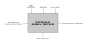
\includegraphics[width=\textwidth,clip=true]{img/IDEF0-1.png}
	\caption{Комплексная диаграмма IDEF0}
\end{figure}

\begin{figure}[H]
	\centering
	
\includegraphics[width=\textwidth,clip=true]{img/IDEF0-2.png}
	\caption{Декомпозиция комплексной диаграммы IDEF0}
\end{figure}

\subsection{IDEF3}

Методология IDEF3 –-- это методология описания процессов. В отличие от IDEF0 она
рассматривает последовательность выполнения задач, а также причинно-следственные
связи между ними \cite{idef3}. Диаграммы IDEF3 состоят из блоков, описывающих функции,
стрелок-связей и перекрёстков, которые показывают, как именно выполняются
процессы.

\obj{Блок} (функциональный элемент) представляет собой прямоугольник, разделенный на
три другие прямоугольника: один большой наверху и два маленьких друг рядом с
другом внизу. В верхнем прямоугольнике содержится имя функции, в нижнем левом
номер его выполнения, в нижнем правом, при необходимости, находится ссылка на
другую функцию. Связи бывают простыми, относительными и связями с условием.

Перекрёстки подразделяются на следующие типы: \obj{И}, \obj{ИЛИ},
\obj{синхронное И}, \obj{синхронное ИЛИ}, а также \obj{исключающее ИЛИ}.

\begin{figure}[H]
	\centering
	
\includegraphics[width=\textwidth,clip=true]{img/IDEF3.png}
	\caption{IDEF3 диаграмма}
\end{figure}

\subsection{DFD}

\term{Диаграммы потоков данных} (англ. \term{DFD}) –-- это способ представления
процессов обработки информации. Они показывают, как информация перемещается из
одной функции к другой. Подобное представление потока данных отражает движение
объектов, их хранение и распространение.

DFD состоит из следующих компонентов: внешняя сущность, процесс, поток данных и
хранилище данных \cite{dfd}. Внешняя сущность представляет собой источник или приёмник
информации и изображается прямоугольником с прямыми углами. Процессы в DFD – это
функции системы, преобразующие входы и выходы, которые изображаются как
прямоугольники со скругленными углами. Потоки данных изображаются стрелками.
Если стрелка соединяет какую-либо функцию с хранилищем данных, то на ней должно
быть отображено имя, отражающее содержание данного потока. Хранилище данных
является прообразом базы данных и изображается как прямоугольник без правой
стороны.

\begin{figure}[H]
	\centering
	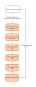
\includegraphics[height=0.8\textwidth,keepaspectratio,clip=true]{img/DFD.png}
	\caption{DFD диаграмма}
\end{figure}

\subsection{UML}

\term{UML} является унифицированным языком моделирования, объекты в котором это
упрощенное представление предметов окружающего нас мира \cite{hunt}. Его используют при
разработке ПО для моделирования бизнес-процессов, системного проектирования и
отображения организационных структур \cite{fowler}. UML диаграммы подразделяются на два типа:
структурные и поведенческие.

\subsubsection{Диаграмма пакетов}

\term{Диаграмма пакетов} --- это структурная диаграмма UML, которая показывает
структуру проектируемой системы на уровне пакетов \cite{martin}. Обычно на диаграмме
изображаются следующие элементы: пакет, пакетированный элемент, зависимость,
импортируемый элемент, импорт пакета, объединение пакета.

\begin{figure}[H]
	\centering
	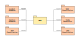
\includegraphics[width=\textwidth,clip=true]{img/UML-package.png}
	\caption{Диаграмма пакетов UML}
\end{figure}

\subsubsection{Диаграмма компонентов}

\term{Диаграмма компонентов} показывает компоненты, предоставляемые и требуемые
интерфейсы, порты и отношения между ними \cite{buch}. Этот тип диаграмм используется в
компонентно-ориентированной разработке для описания систем с
сервисно-ориентированной архитектурой \cite{douglass}.

Компонентно-ориентированная разработка основана на предположения, что ранее
сконструированные компоненты могут быть переиспользованы или, при необходимости,
заменены на некие ``эквивалентные'' или ``совместимые'' компоненты.

\begin{figure}[H]
	\centering
	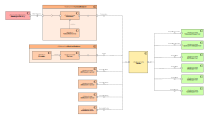
\includegraphics[width=\textwidth,clip=true]{img/UML-components.png}
	\caption{Диаграмма компонентов UML}
\end{figure}

\subsubsection{Диаграмма потока информации}

\term{Диаграмма потока информации} --- это поведенческая диаграмма UML, которая
показывает обмен информацией между сущностями системы на высоком уровне
абстракции. Потоки информации могут быть полезны для описания циркуляции
информации через систему через представление аспектов модели, которые еще не
полностью специфицированы или недостаточно детализированы.

Потоки информации не показывают природу информации, механизмы передачи, порядок
обмена или какие-либо контрольные условия \cite{penker}. Единицы информации могут быть
использованы для представления информации, которая протекает через систему
вместе с информационными потоками еще прежде, чем их реализация будет
проработана.

\begin{figure}[H]
	\centering
	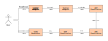
\includegraphics[scale=1.35,clip=true]{img/UML-information-flow.png}
	\caption{Диаграмма потока информации UML}
\end{figure}

\clearpage
\section{Выбор средств разработки}

Так как для компилятора требуется возможность скомпилировать самого себя, то
выбор реализации языка становится очевиден --- это язык C стандарта ISO/IEC
9899:1999.

Кроме того, из соображений минимизации зависимостей для более полного понимания
всего процесса компиляции единственной зависимостью компилятора будет
использование функций GNU C Library, реализующих POSIX-совместимые регулярные
выражения, которые не входят в используемый стандарт языка.

В рамках реализации компилятора не ставится задача реализации собственного
движка регулярных выражений, так как это довольно простая математическая модель
(регулярные языки), разработка которых лишь усложнит код компилятора, который мы
стараемся сделать максимально простым.

Для облегчения процесса сборки приложения в качестве средств систем сборки будет
использован такой инструмент как GNU Make.

В качестве компилятора может быть использован любой компилятор, который
поддерживает стандарт ISO/IEC 9899:1999. Более того, использование разных
компиляторов позволит убедится, что исходный код компилятора соответствует
используемому стандарту.

\clearpage
\section{Оценка стоимости работ}

Варианты использования описывают основные процедуры работы с системой, поэтому
путём их анализа можно определить сложность системы, а, значит, и затраты,
необходимые для её разработки. Во многих случаях исследование вариантов
использования проще, чем поиск функциональных точек, необходимых для работы
других методов оценивания затрат, таких как COCOMO II и Functional Points.

Сложность системы при этом определяется следующими факторами:

\begin{itemize}
	\item количество и сложность действующих лиц, участвующих в варианте использования;

	\item дополнительные требования, такие как многозадачность, безопасность и
		производительность;

	\item внешние факторы, такие как опыт членов команды разработчиков.
\end{itemize}

В качестве единицы сложности системы используется прецедентная точка (Use-Case
Point, UCP), количество таких точек для каждого варианта использования
определяется по формуле:

\begin{equation}
	\mathrm{UCP} = \mathrm{TCP} \times \mathrm{ECF} \times \mathrm{UUCP} \times \mathrm{PF}
\end{equation}

\begin{itemize}
	\item UCP – количество прецедентных точек;
	\item TCP – коэффициент технической сложности;
	\item ECF – коэффициент сложности взаимодействия с окружающей средой;
	\item PF – эффективность работы разработчиков;
	\item UUCP – количество нескорректированных прецедентных точек.
\end{itemize}

Значение UUCP определяется числом шагов, необходимых для выполнения варианта
использования, действующими лицами каждого варианта и общим количеством, и
сложностью вариантов использования рассматриваемом варианте использования 3
шага. Сложность варианта использования определяется в соответствие со следующими
правилами:

\begin{itemize}
	\item \textit{простой} (5 баллов) – предполагается простой пользовательский интерфейс
		и работа не более, чем с одной сущностью базы данных; количество шагов не
		превышает 3, а в реализации задействовано не более 5 классов;

	\item \textit{средней сложности} (10 баллов) – более сложный пользовательский
		интерфейс, работа с двумя или более сущностями базы данных; количество шагов
		составляет от 4 до 7, в реализации задействовано 5-10 классов;

	\item \textit{сложный} (15) – сложная обработка запросов пользователя, работа с тремя и
		более сущностями базы данных; количество шагов превышает 7, количество
		классов в реализации более 10.
\end{itemize}

Варианты использования:

\begin{itemize}
	\item \textit{простой}: выполнение лексического анализа единицы трансляции;
		выполнение синтаксического анализа, вывод диагностических сообщений о
		лексических ошибках в программе;

	\item \textit{средней}: построение AST по дереву разбора, вывод
		диагностических сообщений о синтаксических и лексических ошибках;

	\item \textit{сложный}: построение трехадресного кода, построение SSA, кодогенерация
		кода под целевую платформу.
\end{itemize}

\begin{equation}
	\mathrm{UUCW} = 3 \times 5 + 2 \times 10 + 3 \times 15 = 80
\end{equation}

Действующие лица также разделяются на три класса по следующим правилам:

\begin{itemize}
	\item \textit{простое действующее лицо} (1 балл) – сторонняя система, обращающаяся к
		нашей системе через программный интерфейс;

	\item \textit{действующее лицо средней сложности} (2 балла) – сторонняя система,
		обращающаяся к нашей по сети;

	\item \textit{сложное действующее лицо} (3 балла) – пользователь системы.
\end{itemize}

После этого подсчитывается количество действующих лиц в каждом классе,
количество умножается на соответствующие баллы. В результате получается
нескорректированный вес действующих лиц (UAW). В нашем варианте одно сложное
действующее лицо --- пользователь.

\begin{equation}
	\mathrm{UAW} = 1 \times 3 = 3.
\end{equation}

Значение UUCP вычисляется по формуле:

\begin{equation}
	\mathrm{UUCP} = \mathrm{UUCW} + \mathrm{UAW} = 80 + 3 = 83.
\end{equation}

Для вычисления TCF сначала каждому фактору присваивается вес в зависимости от
того, насколько сильно его влияние на систему (от 0 до 5). После этого
оценивается сложность, связанная с данным фактором (также от 0 до 5). Полученные
значения перемножаются, результаты складываются и получают значение PreTCF
(см. таблицу 1).

\begin{table}[H]
	\caption{Получение значения PreTCF}

	\resizebox{\textwidth}{!}{
		\begin{tabular}{|Sl|Sl|Sl|Sl|}
			\hline
				\multicolumn{1}{|c|}{Описание} &
				\multicolumn{1}{|c|}{Вес} &
				\multicolumn{1}{|c|}{Сложность} &
				\multicolumn{1}{|c|}{Вес × сложность} \\
			\hline
			Распределённая система & 0 & 5 & 0 \\
			Производительность & 0 & 4 & 0 \\
			Эффективность взаимодействия с пользователем & 5 & 3 & 15 \\
			Сложные алгоритмы обработки данных & 5 & 5 & 25 \\
			Возможность повторного использования & 5 & 5 & 25 \\
			Простота установки & 5 & 2 & 10 \\
			Простота использования & 5 & 3 & 15 \\
			Переносимость & 0 & 5 & 0 \\
			Простота модификации & 5 & 5 & 25 \\
			Многозадачность & 0 & 5 & 0 \\
			Безопасность & 0 & 4 & 0 \\
			Открытость для сторонних приложений & 5 & 4 & 20 \\
			Необходимость специальных навыков пользователей & 5 & 1 & 5 \\

			\hline
			PreTCF & \multicolumn{2}{|c|}{} & 144 \\
			\hline
		\end{tabular}
	}
\end{table}

Значение TCF вычисляется по формуле:

\begin{equation}
	\mathrm{TCF} = 0.6 + 0.01 \times \mathrm{PreTCF} = 0.6 + 1.44 = 2.04.
\end{equation}

Аналогичным образом вычисляется значение PreECF (см. таблицу 2).

\begin{table}[H]
	\caption{Получение значения PreECF}

	\resizebox{\textwidth}{!}{
		\begin{tabular}{|Sl|Sl|Sl|Sl|}
			\hline
				\multicolumn{1}{|c|}{Описание} &
				\multicolumn{1}{|c|}{Вес} &
				\multicolumn{1}{|c|}{Сложность} &
				\multicolumn{1}{|c|}{Вес × сложность} \\
			\hline
			Знакомство с UML & 1 & 1 & 1 \\
			Знакомство с предметной областью & 4 & 5 & 20 \\
			Знакомство с объектно-ориентированными технологиями & 3 & 2 & 6 \\
			Опыт ведущего аналитика & 2 & 3 & 6 \\
			Мотивация & 2 & 3 & 6 \\
			Постоянство требований & 1 & 1 & 1 \\
			Наличие совместителей & 0 & 3 & 0 \\
			Трудный язык программирования & 2 & 3 & 6 \\

			\hline
			PreECF & \multicolumn{2}{|c|}{} & 46 \\
			\hline
		\end{tabular}
	}
\end{table}

Значение ECF вычисляется по формуле:

\begin{equation}
	\mathrm{ECF} = 1.4 + (-0.03 \times \mathrm{PreECF}) = 1.4 - 1.38 = 0.02.
\end{equation}

Значение PF определяется как количество человеко-часов, необходимых для
реализации одного варианта использования. Данное значение определяется из опыта
выполнения предыдущих проектов. Если такой опыт отсутствует, то берётся число из
интервала от 15 до 30, обычно 20. Тогда:

\begin{equation}
	\mathrm{UCP} = 83 \times 2.04 \times 0.02 \times 20 \approx 67.60.
\end{equation}

Получили, что для реализации системы потребуется 67.60 человеко-часов.

\gostStructureElement{Заключение}

Таким образом, по итогу проделанной работы сделано следующее:

\begin{itemize}
	\item Изучена предметная область, проведен её анализ, определены цели и
		задачи системы.

	\item Сформулировано словесное описание разрабатываемой информационной
		системы.

	\item Изучены графические нотации методологий IDEF0, IDEF3, DFD и UML,
		их принципы построения, а также построены соответствующие
		модели, описывающие работу данной системы.

	\item Произведено оценивание стоимости создания информационной системы и
		выявлено, сколько потребуется человеко-часов для создания данной
		системы.
\end{itemize}

\clearpage
\printbibliography[heading=bibintoc,title=СПИСОК ИСПОЛЬЗОВАННЫХ ИСТОЧНИКОВ]

\gostStructureElement{Приложение А}
\addtocontents{toc}{\protect\setcounter{tocdepth}{-1}}
\setcounter{section}{0}

\begin{center}
	\textbf{САРАТОВСКИЙ ГОСУДАРСТВЕННЫЙ ТЕХНИЧЕСКИЙ УНИВЕРСИТЕТ ИМЕНИ ГАГАРИНА
	Ю.А.}

	\bigskip
	\bigskip
	\bigskip
	\bigskip

	\begin{table}[H]
		\begin{tabular}{S{p{0.5\textwidth}}S{p{0.5\textwidth}}}
				\multicolumn{1}{c}{УТВЕРЖДАЮ} &
				\multicolumn{1}{c}{УТВЕРЖДАЮ} \\

				Руководитель (должность, наименование предприятия --- заказчика АС) &
				Руководитель (должность, наименование предприятия --- заказчика АС) \\

				Личная подпись Расшифровка подписи &
				Личная подпись Расшифровка подписи \\

				Печать & Печать \\
				Дата & Дата
			\end{tabular}
	\end{table}

	\textbf{Программного обеспечения \enquote{Компилятор языка C}}

	\textbf{ТЕХНИЧЕСКОЕ ЗАДАНИЕ}

	На 21 листе
	
	Действует с \enquote{\_\_\_} \_\_\_\_\_\_\_\_ 2021 г.
\end{center}

\bigskip
\bigskip

\begin{flushleft}
	СОГЛАСОВАНО \\
	Руководитель (должность, наименование согласующей организации) \\
	Личная подпись Расшифровка подписи \\
	Печать \\
	Дата \\
\end{flushleft}

\vfill

\begin{center}
	Саратов 2021
\end{center}

\clearpage
\section{ОБЩИЕ ПОЛОЖЕНИЯ}

\subsection{Полное наименование системы и ее условное обозначение}

Полное наименование системы: \enquote{Автоматизированная информационная система “Компилятор языка C”}.

Краткое наименование системы: АИС \enquote{Компилятор}.

\subsection{Номер договора (контракта)}

Шифр темы: АИС-КА-ФА-07.

Номер контракта: №1/11-11-11-001 от 29.09.2021.

\subsection{Наименования организации-заказчика и\\организаций-участников работ}

Заказчиком системы является Саратовский Государственный технический университет
имени Гагарина Ю.А. Адрес заказчика: 410054, г. Саратов, ул. Политехническая, д.
77.

Разработчиком системы является Нефедов Данил Вадимович. Адрес разработчика:
415011, г. Саратов, ул. Московская, д. 27.

\subsection{Перечень документов, на основании которых создается система}

Основанием для разработки компилятора \enquote{\textit{CC99}} являются следующие
документы и нормативные акты:

\begin{itemize}
	\item ISO/IEC 9989:1999. Programming languages --- C.
	\item Intel® 64 and IA-32 Architectures Software Developer’s Manual, Volume 1:
		Basic Architecture.
	\item The Intel® 64 and IA-32 Architectures Software Developer’s Manual,
		Volumes 2A, 2B, 2C \& 2D: Instruction Set Reference.
	\item The Intel® 64 and IA-32 Architectures Software Developer’s Manual,
		Volumes 3A, 3B, 3C \& 3D: System Programming Guide.
	\item The Intel® 64 and IA-32 Architectures Software Developer’s Manual,
		Volume 4: Model-Specific Registers.
	\item System V Application Binary Interface. AMD64 Architecture Processor
		Supplement (With LP64 and ILP32 Programming Models).
	\item IEEE Std 1003.1-2017.
	\item ISO/IEC JTC 1 Working Group. Rationale for International Standard ---
		Programming Languages --- C.
	\item Documentation for GNU binutils 2.37.
\end{itemize}

\subsection{Плановые сроки начала и окончания работы по созданию системы}

Плановый срок начала работ по созданию АИС \enquote{Компилятор} --- 29 сентября 2021 года.

Плановый срок окончания работ по созданию АИС \enquote{Компилятор} --- 28 февраля 2022 года.

\subsection{Порядок оформления и предъявления заказчику результатов работ по
созданию системы}

Исходный код разработанного программного обеспечения, список технических средств
к закупке, а также инструкция по установке, настройке, запуске рабочего
окружения и его сопровождение должна быть передана Заказчику в установленные им
сроки. Приёмка и проверка работоспособности системы будет осуществлена
комиссией, сформированной заказчиком.

\subsection{Перечень нормативно-технических документов,\\методических материалов,
использованных при\\разработке ТЗ}

При создании и разработки программного обеспечения и проектно-\\эксплуатационной
документации необходимо руководствоваться требованиями следующий документов:

\begin{itemize}
	\item ГОСТ 34.602-89.
\end{itemize}

\subsection{Определения, обозначения и сокращения}

\begin{table}[H]
	\resizebox{\textwidth}{!}{
		\begin{tabular}{|Sl|Sl|}
			\hline
				\multicolumn{1}{|c|}{Сокращение} &
				\multicolumn{1}{|c|}{Расшифровка} \\
			\hline
			ТЗ & Техническое задание \\
			АИС & Автоматизированная информационная система \\
			ЯП & Язык программирования \\
			ABI & Application Binary Interface \\
			AST & Abstract Syntax Tree, абстрактное синтаксическое дерево \\
			3AC & Three Address Code \\
			SSA & Static Single Assignment form \\
			\hline
		\end{tabular}
	}
\end{table}

\clearpage
\section{НАЗНАЧЕНИЕ И ЦЕЛИ СОЗДАНИЯ СИСТЕМЫ}

\subsection{Назначение системы}

АИС \enquote{Компилятор} создается для образовательных целей и предназначена для
обучения студентов и прочих желающих внутреннему устройству и построению в
частности компиляторов, а в общем случае --- программ\-/трансляторов с одного языка
программирования в другой.

\subsection{Цели создания системы}

Основными целями создания АИС \enquote{Компилятор} являются:

\begin{itemize}
	\item Создание компилятора языка C, который полностью или частично
		соответствует международному стандарту ISO/IEC 9899:1999.
	\item Создание компилятора, который поможет студентам и прочим желающим
		разобраться в работе программ-компиляторов и программ\-/трансляторов с одного
		ЯП в другой.
	\item Создание компилятора, который сможет скомпилировать сам себя (так
		называемая раскрутка, англ. \textit{bootstrapping}).
\end{itemize}

Для реализации поставленных целей система должна решать следующие задачи:

\begin{itemize}
	\item Переводить программу, написанную на ЯП C версии определенной и описанной
		в международном стандарте ISO/IEC 9899:1999 в язык ассемблера GNU Assembler
		с синтаксисом AT\&T для архитектуры Intel® 64 в соответствии System V ABI.
	\item Иметь простой и понятный исходный код.
	\item Быть простой в использовании.
	\item Иметь возможность скомпилировать саму себя.
\end{itemize}

\clearpage
\section{ТРЕБОВАНИЯ К СИСТЕМЕ}

\subsection{Требования к системе в целом}

\subsubsection{Требования к структуре и функционированию системы}

\paragraph{Перечень подсистем, их назначение и основные\\характеристики}

В состав АИС \enquote{Компилятор} должны входить следующие подсистемы:

\begin{itemize}
	\item Подсистема лексического анализа (лексический анализатор).
	\item Подсистема синтаксического анализа (синтаксический анализатор).
	\item Подсистема построения AST.
	\item Подсистема перевода AST в 3AC.
	\item Подсистема перевода 3AC в SSA.
	\item Подсистема перевода SSA в код ассемблера GNU Assembler с синтаксисом AT\&T для архитектуры Intel® 64 в соответствии с System V ABI.
\end{itemize}

Подсистема лексического анализа предназначена для а) разбиения исходного кода
входной программа, представленного в качестве массива байт в определенной
кодировке, на отдельные лексические единицы ЯП C; б) выявления и диагностики
лексических ошибок во входной программе.

Подсистема синтаксического анализа предназначена для а) перевода потока токенов,
полученных от лексического анализатора в синтаксическое дерево по грамматике,
соответствующей грамматике языка C, описанного международным стандартом ISO/IEC
9899:1999; б) выявления и диагностики синтаксических ошибок во входной
программе.

Подсистема построения AST предназначена для а) перевода синтаксического дерева,
полученного от синтаксического анализатора в AST; б) выявления и диагностики
семантических ошибок во входной программе.

Подсистема перевода AST в 3AC предназначена для перевода абстрактного
синтаксического дерева, полученного из подсистемы построения AST, в 3AC.

Подсистема перевода 3AC в SSA предназначена для перевод 3AC, полученного из
предыдущей подсистемы в SSA.

Предназначение подсистемы перевода SSA в код ассемблера GNU Assembler с
синтаксисом AT\&T для архитектуры Intel® 64 в соответствии с System V ABI
очевидно из ее названия.

\paragraph{Требования к способам и средствам связи для\\информационного
обмена между компонентами системы}

Требования не предъявляются.

\paragraph{Требования к характеристикам взаимосвязей создаваемой\\системы
со смежными системами}

АИС \enquote{Компилятор} должна взаимодействовать со следующими смежными системами:

\begin{itemize}
	\item Операционная система.
\end{itemize}

\paragraph{Требования к режимам функционирования системы}

Для АИС \enquote{Компилятор} определены следующие режимы функционирования:

\begin{itemize}
	\item Нормальный режим функционирования.
\end{itemize}

В нормальном режиме функционирования системы АИС \enquote{Компилятор} программное
обеспечение обеспечивает возможность функционирования по запросу пользователя.

\paragraph{Требования по диагностированию системы}

Требования не предъявляются.

\paragraph{Перспективы развития, модернизации системы}

АИС должна иметь возможность дальнейшей модернизации как программного
обеспечения, так комплекса технических средств.

Необходимо предусмотреть возможность добавления одного или нескольких проходов
оптимизации SSA; возможность добавления других бэкендов компилятора --- то есть
генерация другого ассемблерного кода, кода для другой архитектуры и/или ABI.

\subsubsection{Требования к численности и квалификации персонала системы}

Для эксплуатации АИС \enquote{Компилятор} определены следующие роли:

\begin{itemize}
	\item Пользователь.
\end{itemize}

Основными возможностями пользователя являются:

\begin{itemize}
	\item Компиляция исходной программы.
	\item Просмотр промежуточных стадий трансляции.
\end{itemize}

Пользователи системы должны иметь опыт работы с любой командной оболочкой совместимой со стандартом IEEE Std 1003.1-2017.

\subsubsection{Показатели назначения}

Требования на время отклика системы не налагаются и зависят от входных данных,
переданных системе на обработку.

Система должна предусматривать возможность масштабирования по производительности
и объему обрабатываемой информации без модификации ее программного обеспечения
путем модернизации используемого комплекса технических средств.

\subsubsection{Требования к надежности}

Требования к надежности не предъявляются, так как это позволит сильно упростить
исходный код АИС для понимания.

Система не обязана сохранять работоспособность и обеспечивать восстановление
своих функций при возникновении каких-либо внештатных ситуаций.

\subsubsection{Требования к эргономике и технической эстетике}

АИС не должна иметь визуальный графический интерфейс. Все взаимодействие с АИС должно производится из командной оболочки соответствующей стандарту IEEE Std 1003.1-2017.

\subsubsection{Требования к транспортабельности для подвижных АС}

Требования не предъявляются.

\subsubsection{Требования к эксплуатации, техническому обслуживанию,\\ремонту и
хранению компонентов системы}

Система должна быть рассчитана на эксплуатацию на персональных компьютерах пользователей.

\subsubsection{Требования к защите информации от несанкционированного\\доступа}

Требования не предъявляются.

\subsubsection{Требования по сохранности информации при авариях}

Требования не предъявляются.

\subsubsection{Требования к защите от влияния внешних воздействий}

Требования не предъявляются.

\subsubsection{Требования к патентной чистоте}

Разработка системы должна осуществляться в рамках рекомендаций по стандартизации Р50.1.028-2001 \enquote{Информационные технологии поддержки жизненного цикла продукции. Методология функционального моделирования}.

\subsubsection{Требования по стандартизации и унификации}

\begin{itemize}
	\item ГОСТ 18421-93.
	\item ГОСТ 19.001-77.
	\item ГОСТ 19.005-85.
	\item ГОСТ 19.402-78.
	\item ГОСТ Р 51904-2002.
\end{itemize}

\subsubsection{Дополнительные требования}

Дополнительные требования не предъявляются.

\subsection{Требования к функциям (задачам), выполняемым\\системой}

\subsubsection{Подсистема лексического анализа}

Подсистема лексического анализа должна разбивать исходный код входной программы,
представленной в качестве массива байт в определенной кодировке, на отдельные
лексические единицы ЯП C.

Подсистема лексического анализа должна предоставлять возможность экспортировать
результат своей работы (полученный поток токенов) в произвольном формате.

Также для подсистемы допускается выявление и диагностика лексических ошибок во
входной программе с выводом диагностических сообщений пользователю, что
соответствует требованиям ISO/IEC 9899:1999.

\subsubsection{Подсистема синтаксического анализа}

Подсистема синтаксического анализа должна переводить потока токенов, полученных
от лексического анализатора в синтаксическое дерево по грамматике,
соответствующей грамматике языка C, описанного международным стандартом ISO/IEC
9899:1999.

Подсистема лексического анализа должна предоставлять возможность экспортировать
результат своей работы (полученное синтаксическое дерево) в произвольном
формате.

Также для подсистемы допускается выявление и диагностика синтаксических ошибок
во входной программе с выводом диагностических сообщений пользователю, что
соответствует требованиям ISO/IEC 9899:1999.

\subsubsection{Подсистема построения AST}

Данная подсистема должна переводит синтаксическое дерево, полученное от
синтаксического анализатора в AST.

Также подсистема должна предоставлять возможность экспортировать результат своей
работы (полученное абстрактное синтаксическое дерево) в произвольном формате.

Также для подсистемы допускается выявление и диагностика семантических ошибок во
входной программе с выводом диагностических сообщений пользователю, что
соответствует требованиям ISO/IEC 9899:1999.

\subsubsection{Подсистема перевода AST в 3AC}

Подсистема перевода AST в 3AC должна переводить абстрактное синтаксическое
дерево в 3AC. Также подсистема должна предоставлять возможность экспортировать
результат своей работы (полученный 3AC) в произвольном формате.

\subsubsection{Подсистема перевода 3AC в SSA}

Подсистема перевода 3AC в SSA должна переводить 3AC в SSA. Также подсистема
должна предоставлять возможность экспортировать результат своей работы
(полученный SSA) в произвольном формате.

\subsubsection{Подсистема перевода SSA в код ассемблера}

Подсистема должна переводить SSA в код ассемблера GNU Assembler с синтаксисом
AT\&T для архитектуры Intel® 64 в соответствии с System V ABI. Полученный
результат должен быть выведен пользователю любым способом. Например, с помощью
вывода в стандартный поток вывода или файл, указанный пользователем.

\subsection{Требования к видам обеспечения}

\subsubsection{Требования к математическому обеспечению системы}

Для лексического анализа допустимо и желательно применение готовых библиотек
программных кодов, реализующих функции работы с регулярными выражениями.

Для синтаксического анализа требуется использовать алгоритм рекурсивного спуска
как наиболее простого. Так как грамматика языка C является контекстно-зависимой,
потребуется применение постпроцессинга полученного синтаксического дерева.

\subsubsection{Требования к лингвистическому обеспечению системы}

Исходя из целей, АИС должна быть разработка с применением языка программирования
C версии, соответствующей международному стандарту ISO/IEC 9899:1999. Также
допустимо применение такого языка как GNU Make для создания системы сборки АИС.

Языком взаимодействия с пользователем является английский язык (американский).

Окончательное требования к кодировке входных данных уточняется в процессе
создания программного обеспечения АИС и не обязано быть согласовано с
Заказчиком.

\subsubsection{Требования к программному обеспечению системы}

При проектировании и разработке системы необходимо использовать только
библиотеки программных кодов с открытым исходным кодом.


Базовой программной платформой должна являться POSIX\-/совместимая операционная
система, в которой используется GNU C Library.

\subsubsection{Требования к техническому обеспечению}

Требования к техническому обеспечению не предъявляются.

\subsubsection{Требования к метрологическому обеспечению}

Требования к метрологическому обеспечению не предъявляются.

\clearpage
\section{СОСТАВ И СОДЕРЖАНИЕ РАБОТ ПО\\СОЗДАНИЮ (РАЗВИТИЮ) СИСТЕМЫ}

\begin{table}[H]
		\begin{tabular}{|Sl|S{p{7cm}}|S{p{7cm}}|}
			\hline
				\multicolumn{1}{|c|}{Этап} &
				\multicolumn{1}{|c|}{Содержание работ} &
				\multicolumn{1}{|c|}{Результаты работ} \\
			\hline

			1 &
			Разработка документов технического проекта АИС \enquote{Компилятор} &
			Документы технического проекта АИС \enquote{Компилятор} \\
			\hline

			2 &
			Проектирование, создание и тестирование программного обеспечения АИС \enquote{Компилятор} &
			Программное обеспечение АИС \enquote{Компилятор} \\
			\hline

			3 &
			Приемка АИС \enquote{Компилятор} &
			Акт о приемке АИС \enquote{Компилятор} \\
			\hline
		\end{tabular}
\end{table}

\clearpage
\section{ПОРЯДОК КОНТРОЛЯ И ПРИЕМКИ СИСТЕМЫ}

\subsection{Виды, состав, объем и методы испытаний системы}

Каждая подсистема АИС должна пройти комплексное тестирование для проверки
корректности работы. Должно быть также проведено интеграционное тестирование
каждой подсистемы по отдельности и всех вместе для выявления проблем
взаимодействия как внутри подсистем, так и подсистем между собой.

Кроме того АИС должна пройти инспекцию кода комиссией, в состав которой входят
представители Заказчика и Исполнителя. Инспекция кода должна подтвердить, что
исходный код АИС соответствует предъявляемым к нему требованиям качества.

\subsection{Общие сведения к приемке работ по стадиям}

Сдача-приемка осуществляется комиссией, в состав которой входят представители
Заказчика и Исполнителя. По результатам приемки подписывается акт приемочной
комиссии.

\subsection{Статус приемочной комиссии}

Статус приемочной комиссии определяется Заказчиком до проведения испытаний.

\clearpage
\section{ТРЕБОВАНИЯ К СОСТАВУ И СОДЕРЖАНИЮ\\РАБОТ ПО ПОДГОТОВКЕ ОБЪЕКТА\\
АВТОМАТИЗАЦИИ К ВВОДУ СИСТЕМЫ В\\ДЕЙСТВИЕ}

Требования не предъявляются.

\clearpage
\section{ТРЕБОВАНИЯ К ДОКУМЕНТИРОВАНИЮ}

Требования не предъявляются.

\clearpage
\section{ИСТОЧНИКИ РАЗРАБОТКИ}

Учебники, учебные пособия, научные работы и другие материалы по а) построению
трансляторов кода; б) формальным языкам; в) системному и низкоуровневому
программированию. Документы, приведенные в пункте 1.4.

\end{document}

% 1. ГОСТ 7.32-2017. Система стандартов по информации, библиотечному и
%    издательскому делу. ОТЧЕТ О НАУЧНО-ИССЛЕДОВАТЕЛЬСКОЙ РАБОТЕ. Структура и
%    правила оформления.
% 2. How to set up Russian Cyrillic Times New Roman font in PdfLaTeX?.
%    <https://tex.stackexchange.com/q/405433/225663>.
